%intestazione tipo degli appunti di matematica

\documentclass[a4paper, oneside]{article}
\usepackage[utf8]{inputenc}
\usepackage[italian]{babel}
\usepackage{graphicx}
\usepackage{caption}
	\captionsetup{format=hang,labelfont={sf,bf}}
\usepackage{multicol}
\usepackage{ulem}
\usepackage{lipsum} 
\usepackage[leqno,intlimits]{amsmath}
\usepackage{amssymb}
\usepackage{amsthm}
\usepackage{yhmath}
\usepackage[leqno,fleqn,intlimits]{empheq}
\usepackage{pgfplots}
	\pgfplotsset{/pgf/number format/use comma,compat=newest}
\usepackage{xcolor}
\usepackage{framed}
\usepackage{cancel}
\usepackage{ifthen}
\usepackage{intcalc}
\usepackage[most]{tcolorbox}
\usepackage{forest}
\usepackage{booktabs}

%%%%%%%%%%%%%%%%%%%%%%%%%%%%%%%%%%%%%%%%%%%%%%%%%%%%%%%%%%%%%%%%%%%%%%%%%%%%%%%%%%%%%%%%%%

	% Comandi per la creazione del riquadro attorno alle equazioni
	\newif\ifmarg
	\margtrue
	\ifmarg
	\makeatletter
	\let\mytagform@=\tagform@
	\def\tagform@#1{\maketag@@@{\mbox{~}\hbox{\rlap{\hspace{0.5in}(\ignorespaces#1\unskip\@@italiccorr)}}}\kern1sp}
	\renewcommand{\eqref}[1]{{\mytagform@{\ref{#1}}}}
	\makeatother
	\fi
	
	\newcommand*\mygraybox[0]{%
		\tcbhighmath}
		
	\newcommand{\equazione}[1]{	\begin{empheq}[box=\mygraybox]{equation*}
			#1
		\end{empheq}}
	%%%%%%%%%%%%%%%%%%%%%%%%%%%%%%%%%%%%%%%%%%%%%%%%%%%%%%%%%%%%%%%%%%%
	% Creazione dell'ambiente ``NOTA'' 
		\newlength\sidebar
		\newlength\envrule
		\newlength\envborder
		\setlength\sidebar{1.5mm}
		\setlength\envrule{0.4pt}
		\setlength\envborder{2.5mm}
		
		\makeatletter
		\long\def\fboxs#1{%
		  \leavevmode
		  \setbox\@tempboxa\hbox{%
		    \color@begingroup
		      \kern\fboxsep{#1}\kern\fboxsep
		    \color@endgroup}%
		  \@frames@x\relax}
		\def\frameboxs{%
		  \@ifnextchar(%)
		    \@framepicbox{\@ifnextchar[\@frameboxs\fboxs}}
		\def\@frameboxs[#1]{%
		  \@ifnextchar[%]
		    {\@iframeboxs[#1]}%
		    {\@iframeboxs[#1][c]}}
		\long\def\@iframeboxs[#1][#2]#3{%
		  \leavevmode
		  \@begin@tempboxa\hbox{#3}%
		    \setlength\@tempdima{#1}%
		    \setbox\@tempboxa\hb@xt@\@tempdima
		         {\kern\fboxsep\csname bm@#2\endcsname\kern\fboxsep}%
		    \@frames@x{\kern-\fboxrule}%
		  \@end@tempboxa}
		\def\@frames@x#1{%
		  \@tempdima\fboxrule
		  \advance\@tempdima\fboxsep
		  \advance\@tempdima\dp\@tempboxa
		  \hbox{%
		    \lower\@tempdima\hbox{%
		      \vbox{%
		        %\hrule\@height\fboxrule
		        \hbox{%
		         \vrule\@width\fboxrule
		          #1%
		          \vbox{%
		            \vskip\fboxsep
		            \box\@tempboxa
		            \vskip\fboxsep}%
		          #1%
		          }%\vrule\@width\fboxrule}%
		        }%\hrule\@height\fboxrule}%
		                          }%
		        }%
		}
		\def\esefcolorbox#1#{\esecolor@fbox{#1}}
		\def\esecolor@fbox#1#2#3{%
		  \color@b@x{\fboxsep\z@\color#1{#2}\fboxs}{\color#1{#3}}}
		\makeatother
		
		\definecolor{exampleborder}{rgb}{0.5, 0.5, 0.5}
		\definecolor{examplebg}{rgb}{0.89, 0.89, 0.89}
		\definecolor{statementborder}{rgb}{.9,0,0}
		\definecolor{statementbg}{rgb}{1,.9,.9}
		
		\newenvironment{eseframed}{%
		  \def\FrameCommand{\fboxrule=\the\sidebar  \fboxsep=\the\envborder%
		  \esefcolorbox{exampleborder}{examplebg}}%
		  \MakeFramed{\FrameRestore}}%
		 {\endMakeFramed}
		
		\newenvironment{nota}[1]
		{\par\medskip%\refstepcounter{esempio}%
		\hbox{%
		\fboxsep=\the\sidebar\hspace{-\envborder}\hspace{-.5\sidebar}%
		\colorbox{exampleborder}{%
		\hspace{\envborder}\footnotesize\sffamily\bfseries%
		\textcolor{white}{{{\large
		#1}}\hspace{\envborder}}
		}
		}
		\nointerlineskip\vspace{-\topsep}%
		\begin{eseframed}\noindent\ignorespaces%
		}
		{\end{eseframed}\vspace{-\baselineskip}\medskip}
	%%%%%%%%%%%%%%%%%%%%%%%%%%%%%%%%%%%%%%%%%%%%%%%%%%%%%%%
	\newcounter{tartaglia}
	\newcounter{newton}
	\newcounter{i}% contatore delle righe
	\newcounter{j}% contatore delle colonne
	\newcounter{n}% è il numero massimo di righe
	\newcounter{I}% contatori di servizio
	\newcounter{J}%
	
	%creazione del comando ``cbinomiale''
	\newcommand{\cbinomiale}[2]{%
		\intcalcDiv{\intcalcFac{#1}}{\intcalcMul{\intcalcFac{#2}}{\intcalcFac{\intcalcSub{#1}{#2}}}}
	}
	
	%creazione del comando ``Binomio di Newton''
		\newcommand{\newton}[1]{%
			\stepcounter{newton}%
			\setcounter{i}{1}%
			\setcounter{j}{0}%
			\setcounter{n}{#1}%
				\begin{center}
				\begin{tikzpicture}[node distance=15 mm]
					\node (\thenewton_n0_0){$\displaystyle\binom{0}{0}$};
					\whiledo{\thei<\then}{%
					\setcounter{I}{\thei}%
					\addtocounter{I}{-1}%
						\whiledo{\thej<\thei}{%
							\setcounter{J}{\thei}%
							\addtocounter{J}{-1}%
								\node[below left of=\thenewton_n\theI_\thej](\thenewton_n\thei_\thej){$\displaystyle\binom{\thei}{\thej}$};
								\stepcounter{j}%
							}
						\node[below right of=\thenewton_n\theI_\theJ](\thenewton_n\thei_\thej){$\displaystyle\binom{\thei}{\thej}$};
						\stepcounter{i}%
						\setcounter{j}{0}%
					}
				\end{tikzpicture}
				\end{center}
	}
		
	%creazione del comando ``Triangolo di Tartaglia''
		\newcommand{\tartaglia}[2]{%
			\stepcounter{tartaglia}%
			\setcounter{i}{1}%
			\setcounter{j}{0}%
			\setcounter{n}{#1}%
				\begin{center}
				\begin{tikzpicture}[node distance=#2 mm]
					\node (\thetartaglia_t0_0){\cbinomiale{0}{0}};
					\whiledo{\thei<\then}{%
					\setcounter{I}{\thei}%
					\addtocounter{I}{-1}%
						\whiledo{\thej<\thei}{%
							\setcounter{J}{\thei}%
							\addtocounter{J}{-1}%
								\node[below left of=\thetartaglia_t\theI_\thej](\thetartaglia_t\thei_\thej){\cbinomiale{\thei}{\thej}};
								\stepcounter{j}%
							}
						\node[below right of=\thetartaglia_t\theI_\theJ](\thetartaglia_t\thei_\thej){\cbinomiale{\thei}{\thej}};
						\stepcounter{i}%
						\setcounter{j}{0}%
					}
				\end{tikzpicture}
				\end{center}
	}

%%%%%%%%%%%%%%%%%%%%%%%%%%%%%%%%%%%%%%%%%%%%%%%%%%%%%%%%%%%%%%%%%%%%%%%%%%%%%%%%%%%%%%%%%%%

%ridefinizione comandi
	\newcommand{\example}{\paragraph{Esempio}}
	\newcommand{\tesi}{\noindent\textit{tesi.}\hspace{1em}}
	\newcommand{\gradi}{$^\text{o}$ }
	\newcommand{\CE}{\text{CE}\hspace{0.5em}}
	\newcommand{\pin}[1]{\frac{\pi}{#1}}
	\newcommand{\modulo}[2]{\Big[#1\Big]_{#2}}
	\newcommand{\pimod}[1]{\Big[#1\Big]_{2\pi}}
	\DeclareMathOperator{\arcsec}{arcsec}
	\DeclareMathOperator{\arccot}{arccot}
	\DeclareMathOperator{\arccsc}{arccsc}
	\newcommand{\R}{\mathbb{R}}
	\newcommand{\mezzo}{\frac{1}{2}}
	\newcommand{\pimezzi}{\frac{\pi}{2}}
	\newcommand{\mm}[1]{$\displaystyle#1$}
	
%definizioni particolari
\newcommand{\straniero}[1]{\textit{#1}} %parole straniere
\newcommand{\titolo}[1]{\textsc{#1}} %titoli
\newcommand{\evid}[1]{\textbf{\textcolor{blue}{#1}}} %parole evidenziate
\newcommand{\salt}{\hspace{1em}[...]} %comando per la creazione dei puntini di sospensione tra quadre

\usepackage[pdftex,
            pdfauthor={Davide Peccioli},
            pdftitle={Relatività},
            pdfsubject={Fisica},
            pdfkeywords={Some Keywords},
            pdfproducer={Latex with hyperref, or other system},
            pdfcreator={pdflatex, or other tool}]{hyperref}
\hypersetup{
	  colorlinks=true,
	  linkcolor=blue,
	  filecolor=blue,
	  citecolor = black,      
	  urlcolor=cyan,
	  }

%%%%%%%%%%%%%%%%%%%%%%%%%%%%%%%%%%%%%%%%%%%%%%%%%%%%%%%%%%%%%%%%%%%%%%%%%%%%%%%%%%%%%%%%%%%

\title{Relatività}
\author{Davide Peccioli}
\date{}

\begin{document}

\maketitle

\tableofcontents

\section{Albert Einstein}

\subsection*{Estratti da \titolo{Come io vedo il mondo}}

\begin{quotation}
Se consideriamo le nostre vite e i nostri sforzi osserviamo, ben presto, che quasi la maggior parte delle nostre azioni e dei nostri desideri è collegata all'esistenza di altri esseri umani. Notiamo che la nostra natura somiglia in tutto a quella degli animali sociali. Mangiamo cibo che altri hanno coltivato, vestiamo abiti fatti da altri, viviamo in case costruite da altri. La più grande parte del nostro sapere e delle nostre convinzioni ci è stata comunicata da altra gente, per mezzo di un linguaggio creato da altri. Senza il linguaggio le nostre capacità sarebbero affatto misere, comparate a quelle degli animali superiori; siamo obbligati perciò ad ammettere che dobbiamo il nostro principale vantaggio sulle bestie al fatto che viviamo in una società umana. L’individuo, se lasciato solo dalla nascita, resterebbe primitivo e bestiale, nei pensieri e nei sentimenti, in una misura che possiamo a stento concepire. L’individuo è quello che è, e il suo significato non gli viene tanto in virtù della sua individualità, ma piuttosto in quanto membro di una grande società umana, che indirizza la sua esistenza materiale e spirituale, dalla culla fino alla tomba.

Il valore di un uomo per la comunità dipende principalmente dal modo con cui i suoi sentimenti, pensieri e azioni sono diretti a promuovere il bene dei suoi simili. Lo consideriamo buono o cattivo secondo questo metro. All'apparenza sembra come se la nostra stima di un uomo dipenda interamente dalle sue qualità sociali.

Eppure un simile atteggiamento sarebbe sbagliato. È chiaro che tutte le cose di valore, materiali, spirituali e morali, che noi riceviamo dalla società, possono essere ricondotte all'origine attraverso innumerevoli generazioni di determinati individui creativi. L’uso del fuoco, la coltivazione di piante commestibili, la macchina a vapore, ogni cosa fu scoperta da un singolo uomo.

Solo l'individuo può pensare, e quindi creare nuovi valori per la società anzi, anche stabilire nuovi modelli morali a cui si conforma la vita della comunità. Senza personalità creative, che pensano e giudicano indipendentemente, il progresso della società è impensabile quanto lo sviluppo della personalità individuale senza il terreno fertile della comunità.

Perciò la salute della società dipende tanto dall'indipendenza degli individui che la compongono, quanto dalla loro stretta coesione politica. È stato detto molto giustamente che  la cultura grecoeuroamericana è un tutt'uno e che in particolare la sua eccezionale fioritura nel Rinascimento italiano, che pose fine alla stagnazione del Medioevo europeo, si fonda sulla liberazione e sul relativo isolamento dell'individuo.

Consideriamo adesso l'epoca in cui viviamo. Come sta la società, come sta l'individuo? La popolazione delle nazioni civilizzate è estremamente densa rispetto al passato. Oggi l'Europa conta circa il triplo di abitanti rispetto a cento anni fa. Ma il numero di grandi uomini è calato in maniera sproporzionata. Solo pochi individui sono noti alle masse come personalità, per i loro risultati creativi. In una certa misura l'organizzazione ha preso il posto del grande uomo, specialmente nel campo tecnico, ma anche in modo tangibile in quello scientifico.

La mancanza di figure eccezionali colpisce particolarmente nel dominio dell' arte. Pittura e musica sono definitivamente degenerate e hanno ampiamente perso il fascino popolare. In politica, non solo mancano i capi, ma l'indipendenza dello spirito e il senso della giustizia dei cittadini sono in larga misura in declino. Il regime democratico e parlamentare, che si basa su questa indipendenza, è stato scosso in molti luoghi, sono sorte dittature e vengono tollerate perché l'umano senso della dignità e dei diritti dell'individuo non è più abbastanza forte. Nel giro di due settimane masse, come greggi, possono essere portate dai giornali a uno stato di furia eccitata tale che gli uomini sono pronti a indossare l'uniforme, a uccidere e a farsi uccidere, in nome delle mire inutili di pochi gruppi interessati. Il servizio militare obbligatorio mi sembra il sintomo più disgraziato di questa mancanza di dignità personale di cui oggi soffre l'umanità civilizzata. Non c'è da meravigliarsi se non mancano coloro che profetizzano la prossima eclissi della nostra civiltà. lo non sono uno di quei pessimisti; credo nell'arrivo di tempi migliori. Lasciatemi brevemente elencare le ragioni di tale mia fiducia.

Secondo me gli attuali sintomi di decadenza si spiegano col fatto che lo sviluppo dell'industria e delle macchine ha reso la lotta per l'esistenza molto più dura, in gran parte a detrimento del libero sviluppo dell'individuo. Ma questo sviluppo delle macchine significa che serve sempre meno il lavoro dell'individuo per la soddisfazione dei bisogni della comunità. Una divisione del lavoro, pianificata, diventa sempre più una necessità impellente e tale divisione porterà alla sicurezza materiale dell'individuo. La sicurezza, il tempo libero e l'energia che l'individuo avrà a sua disposizione potranno servire al suo ulteriore sviluppo. In questo modo la. comunità potrebbe recuperare la sua salute e noi vogliamo sperare che futuri storici spiegheranno i sintomi di malattia della presente società come indisposizione infantile di un' aspirante umanità, dovuta totalmente all'eccessiva velocità con cui la civilizzazione stava avanzando.
\end{quotation}

\subsection*{\titolo{Testamento spirituale}}

\begin{quotation}
In considerazione del fatto che in ogni futura guerra mondiale verrebbero certamente impiegate armi nucleari e che tali armi mettono in pericolo la continuazione stessa dell'esistenza dell'umanità, noi rivolgiamo un pressante appello ai governi di tutto il mondo affinché si rendano conto e riconoscano pubblicamente che i loro obbiettivi non possono essere perseguiti mediante una guerra mondiale e li invitiamo, di conseguenza, a cercare mezzi pacifici per la soluzione di tutte le questioni controverse tra loro.

Nella tragica situazione cui I'umanità si trova di fronte noi riteniamo che gli scienziati debbano riunirsi in conferenza per accertare i pericoli determinati dallo sviluppo delle armi di distruzione in massa e per discutere una risoluzione nello spirito del progetto annesso. Parliamo in questa occasione non come membri di questa o quella Nazione, Continente o Fede, ma come esseri umani, membri della razza umana, la continuazione dell'esistenza della quale è ora in pericolo.

Il mondo è pieno di conflitti e, al di sopra di tutti i conflitti minori, c'e la lotta titanica tra il comunismo e l'anticomunismo. Quasi ognuno che abbia una coscienza politica ha preso fermamente posizione in una o più di tali questioni, ma noi vi chiediamo, se potete, di mettere in disparte tali sentimenti e di considerarvi solo come membri di una specie biologica che ha avuto una storia importante e della quale nessuno di noi può desiderare la scomparsa.

Cercheremo di non dire nemmeno una parola che possa fare appello a un gruppo piuttosto che a un altro. Tutti ugualmente sono in pericolo e se questo pericolo è compreso vi è la Speranza che possa essere collettivamente scongiurato. Dobbiamo imparare a pensare in una nuova maniera: dobbiamo imparare a chiederci non quali passi possono essere compiuti per dare la vittoria militare al gruppo che preferiamo, perché non vi sono più tali passi; la domanda che dobbiamo rivolgerci è: «quali passi possono essere compiuti per impedire una competizione militare il cui esito sarebbe disastroso per tutte le parti?».

L'opinione pubblica e anche molte persone in posizione autorevole non si sono rese conto di quali sarebbero le conseguenze di una guerra con armi nucleari. L'opinione pubblica ancora pensa in termini di distruzione di città. Si sa che le nuove bombe sono più potenti delle vecchie e che mentre una bomba atomica ha potuto distruggere Hiroshima, una bomba all'idrogeno potrebbe distruggere le città più grandi come Londra, New York e Mosca. É fuori di dubbio che in una guerra con bombe all'idrogeno le grandi città sarebbero distrutte; ma questo e solo uno dei minori disastri cui si andrebbe incontro.

Anche se tutta la popolazione di Londra, New York e Mosca venisse sterminata il mondo potrebbe nel giro di alcuni secoli riprendersi dal colpo; ma noi ora sappiamo, specialmente dopo l'esperimento di Bikini, che le bombe nucleari possono gradatamente diffondere la distruzione su un'area molto più ampia di quanto non si supponesse. É stato dichiarato da fonte molto autorevole che ora è possibile costruire una bomba 2500 volte più potente di quella che distrusse Hiroshima.

Una bomba all'idrogeno che esploda vicino al suolo o sott'acqua invia particelle radioattive negli strati superiori dell'aria. Queste particelle si abbassano gradatamente e raggiungono la superficie della terra sotto forma di una polvere o pioggia mortale.

Nessuno sa quale ampiezza di diffusione possano raggiungere queste letali particelle radioattive, ma le maggiori autorità sono unanimi nel ritenere che una guerra con bombe all'idrogeno potrebbe molto probabilmente porre fine alla razza umana.

Si teme che, qualora venissero impiegate molte bombe all'idrogeno, vi sarebbe una morte universale, immediata solo per una minoranza mentre per la maggioranza sarebbe riservata una lenta tortura di malattie e disintegrazione.

Molti ammonimenti sono stati formulati da personalità eminenti della scienza e da autorità della strategia militare.

Nessuno di essi dirà che i peggiori risultati sono certi: ciò che essi dicono è che questi risultati sono possibili e che nessuno può essere sicuro che essi non si verificheranno. Non abbiamo ancora constatato che le vedute degli esperti in materia dipendano in qualsiasi modo dalle loro opinioni politiche e dai loro pregiudizi. Esse dipendono solo, per quanto hanno rivelato le nostre ricerche, dall'estensione delle conoscenze particolari del singolo. Abbiamo riscontrato che coloro che più sanno sono i più pessimisti.

Questo dunque e il problema che vi presentiamo, netto, terribile ed inevitabile: dobbiamo porre fine alla razza umana oppure l'umanità dovrà rinunciare alla guerra?

É arduo affrontare questa alternativa poiché è così difficile abolire la guerra. L'abolizione della guerra chiederà spiacevoli limitazioni della sovranità nazionale, ma ciò che forse più che ogni altro elemento ostacola la comprensione della situazione è il fatto che il termine «umanità» appare vago ed astratto, gli uomini stentano a rendersi conto che il pericolo è per loro, per i loro figli e loro nipoti e non solo per una generica e vaga umanità.

É difficile far sì che gli uomini si rendano conto che sono loro individualmente ed i loro cari in pericolo imminente di una tragica fine.

E cosi sperano che forse si possa consentire che le guerre continuino purché siano vietate le armi moderne. Questa Speranza è illusoria.   

Per quanto possano essere raggiunti accordi in tempo di pace per non usare le bombe all'idrogeno, questi accordi non saranno più considerati vincolanti in tempo di guerra ed entrambe le parti si dedicheranno a fabbricare bombe all'idrogeno non appena scoppiata una guerra, perché se una delle parti fabbricasse le bombe e l'altra no, la parte che le ha fabbricate risulterebbe inevitabilmente vittoriosa.

Sebbene un accordo per la rinuncia alle armi nucleari nel quadro di una riduzione generale degli armamenti non costituirebbe una soluzione definitiva, essa servirebbe ad alcuni importanti scopi.

In primo luogo ogni accordo fra Est e Ovest è vantaggioso in quanto tende a diminuire la tensione internazionale. In secondo luogo l'abolizione delle armi termonucleari se ognuna delle parti fosse convinta della buona fede dell'altra, diminuirebbe il timore di un attacco improvviso del tipo di Pearl Harbour che attualmente tiene entrambe le parti in uno stato di apprensione nervosa.

Saluteremo perciò con soddisfazione un tale accordo, anche se solo come un prime passo. La maggior parte di noi non è di sentimenti neutrali, ma come esseri umani dobbiamo ricordare che perché le questioni fra Est e Ovest siano decise in modo da dare qualche soddisfazione a qualcuno, comunista o anticomunista, asiatico, europeo o americano, bianco o nero, tali questioni non devono essere decise con la guerra.

Desideriamo che ciò sia ben compreso sia in oriente che in occidente. Se vogliamo, possiamo avere davanti a noi un continuo progresso in benessere, conoscenze e saggezza. Vogliamo invece scegliere la morte perché non siano capaci di dimenticare le nostre controversie?

Noi rivolgiamo un appello come esseri umani ad esseri umani: ricordate la vostra umanità e dimenticate il resto. Se sarete capaci di farlo vi è aperta la via di un nuovo Paradiso, altrimenti è davanti a voi il rischio della morte universale.
\end{quotation}

\section{Relatività ristretta}

Verso la fine del XIX secolo la maggior parte degli scienziati era convinta che le leggi fondamentali della fisica fossero state ormai scoperte.

Le equazioni di Newton spiegavano con successo il moto degli oggetti sulla Terra e nei cieli. La \textbf{meccanica newtoniana} era una teoria estremamente solida, che raccoglieva ed inquadrava secoli di osservazioni sul movimento; costituiva inoltre la base per lo studio dei fluidi e delle onde meccaniche e dava, atraverso la teorica cinetica della materia, una spiegazione meccanica per molti fenomeni termici.

La teoria dell'\textbf{elettromagnetismo di Maxwell}, d'altra parte, spiegava in modo unitario e coerente la totalità dei fenomeni elettrici e magnetici, e aveva consentito di riconoscere la natura elettromagnetica della luce.

Queste due basilari teorie mostravano, però una fondamentale contraddizione.

Le leggi di Newton, infatti, si basavano sulla relatività galileiana, secondo cui non c'era alcun sistema di riferimento preferenziale, ma registrando valori diversi delle grandezze fisiche in gioco in base al sistema di riferimento.
Le teorie di Maxwell, invece, prevedevano per la luce il valore costante $c$. Di conseguenza le equazioni di Maxwell erano da considerarsi applicabili solo in un particolare sistema inerziale in cui la velocità della luce fosse uguale a $c$. Questo riferimento avrebbe assunto il carattere di un \textbf{sistema privilegiato}, violando il principio di relatività galileiana.

Si pensò allora di realizzare, utilizzando la luce, un esperimento capace di stabilire se, fra tutti i sistemi inerziali, ce ne fosse uno in quiete assoluta, nel quale la velocità della luce fosse esattamente uguale a $c$. Si pensò che questo sistema di riferimento potesse essere l'etere.

\subsection{Esperimento di Michelson e Morley}

È un esperimento realizzato per rilevare la velocità della Terra rispetto all'etere.

\begin{center}
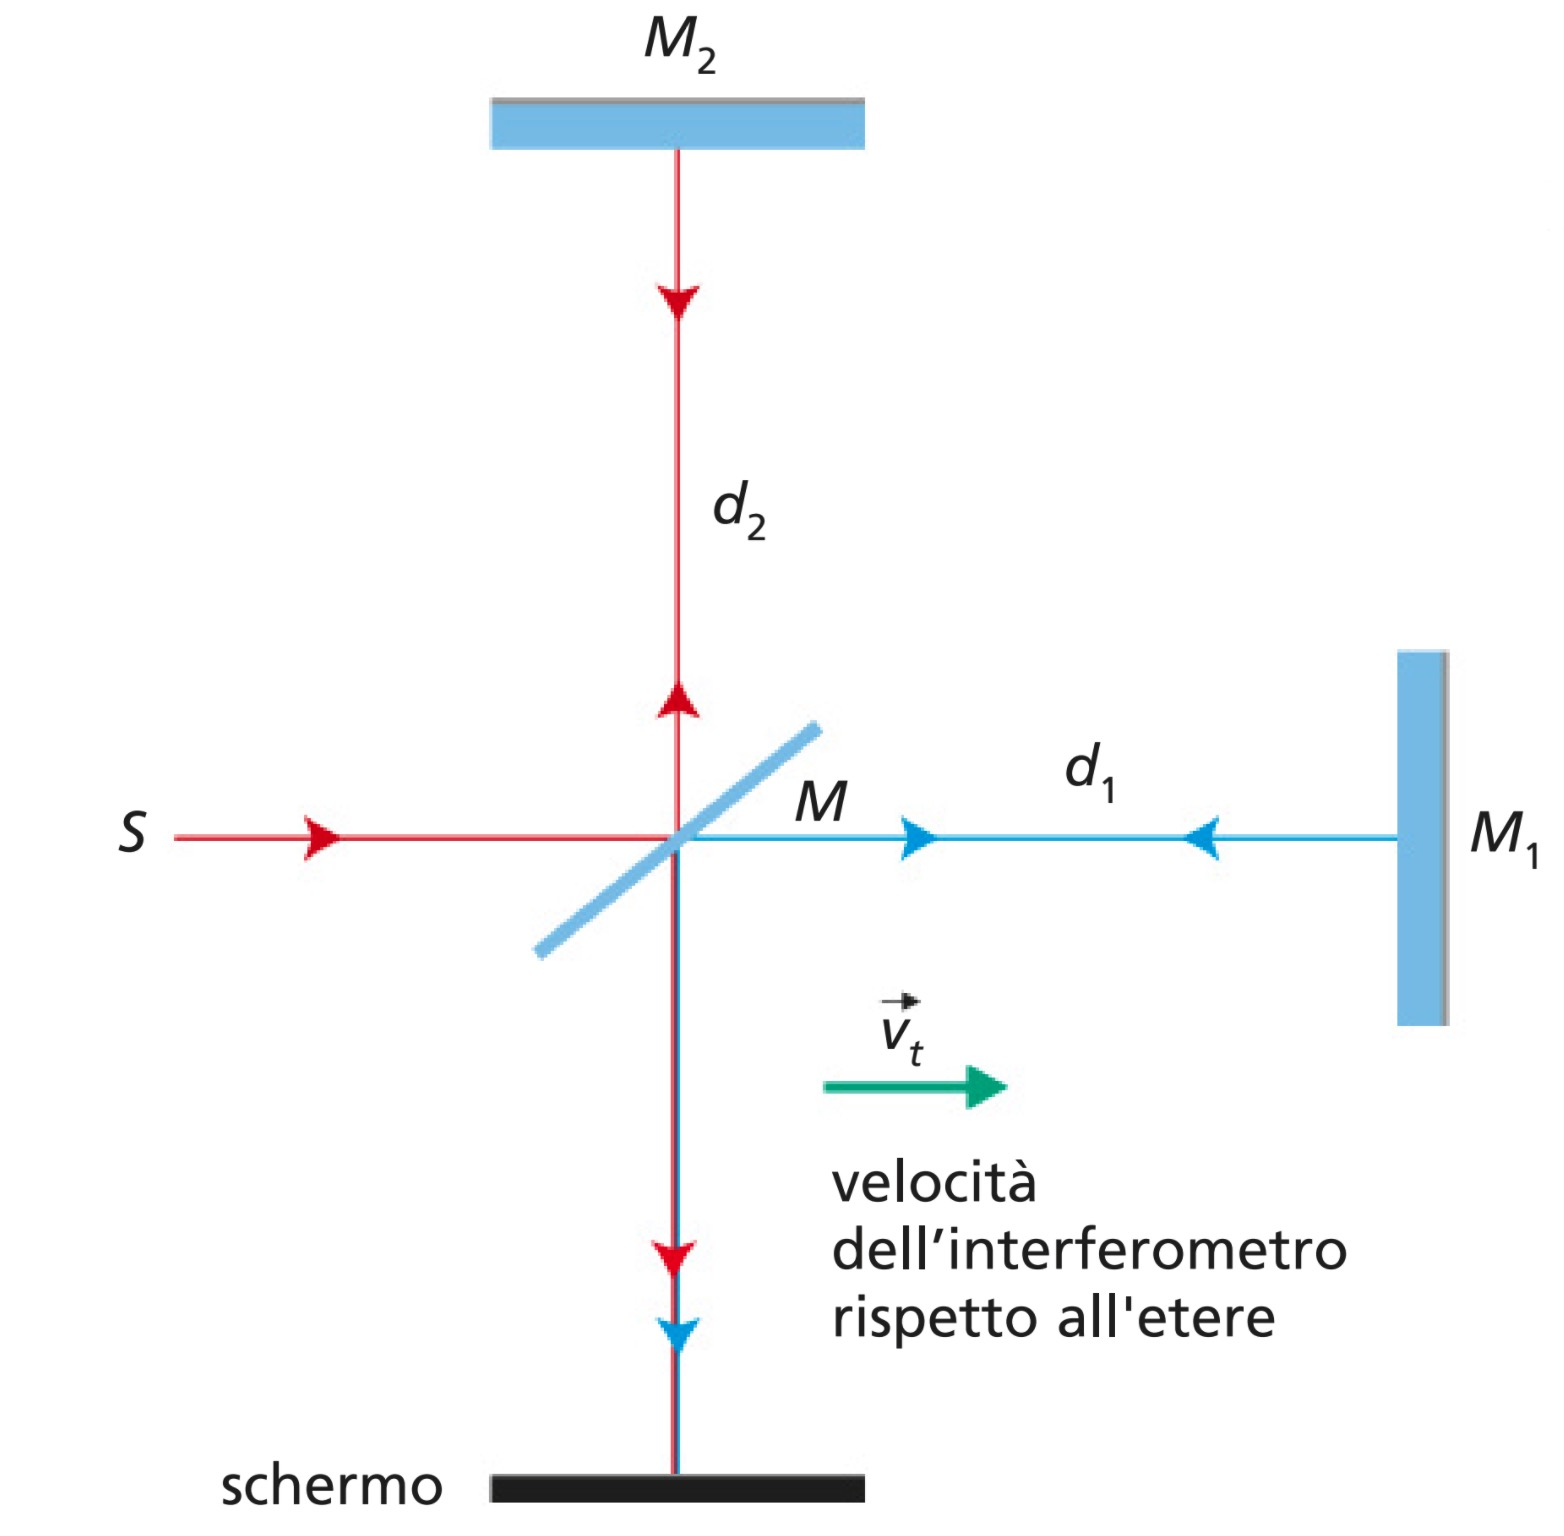
\includegraphics[width=8cm]{img/rrrd}
\end{center}

Un raggio di luce, partendo dalla sorgente $S$, arriva alla lastra di vetro $M$, che in parte riflette il raggio e in parte lo rifrange.
Così facendo i due raggi di luce che si creano, per mezzo di altri specchi, arrivano alla superficie in cui si crea un interferenza.

Ammettendo che la velocità con cui si muove la terra rispetto all'etere sia parallela alla distanza $d_1$, la luce in questo braccio dovrebbe avere una velocità diversa rispetto all'altro braccio.

Ruotando l'interferometro affinché sia il braccio $d_2$ parallelo alla velocità della terra, dovrebbe cambiare la velocità della luce in quel braccio, e quindi modificare le frange di interferenza sullo schermo.

Pur ripetendo l'esperimento numerose volte, in diverse condizioni e in diverse parti del mondo, le frange rimanevano invariate.

\subsection{Postulati della relatività ristretta}

Einstein arriva ad una soluzione per risolvere tutti paradossi creati, stilando due \textbf{postulati}

\begin{nota}{Postulato della relatività}
Le leggi della fisica sono le stesse per tutti i sistemi di riferimento inerziali. Non esiste un sistema di riferimento privilegiato.
\end{nota}

Einstein espande il concetto di Galileo sulle leggi della dinamica a tutte le leggi della fisica

\begin{nota}{Postulato della velocità della luce}
La velocità della luce nel vuoto ha lo stesso valore $c$ in tutte le direzioni e in tutti i sistemi di riferimento inerziali.
\end{nota}

Ci sono diversi esperimenti che permettono di dimostrare la validità di queste affermazioni.
\begin{enumerate}
\item \textbf{Esperimento di Bertozzi} (1964): egli usa il LINAC per accelerare diverse particelle, notando che ad un certo punto $v$ raggiunge un certo valore limite (appunto $c$), mentre l'energia cinetica $k$ no. Questo dimostra la validità delle teorie di Einstein.
\item \textbf{Esperimento dei Pioni}: i pioni decadono in due fotoni (che hanno velocità della luce); si misura la velocità del fotone sia rispetto al laboratorio che rispetto al pione: le due velocità sono uguali, dimostrando che la velocità della luce è uguale in tutti i sistemi di riferimento.
\end{enumerate}

Se le leggi della fisica hanno la stessa forma e la velocità della luce lo stesso valore in tutti i sistemi di riferimento, solo altre le grandezze che, in questa teoria, diventano variabili, dipendenti dal riferimento.

\subsection{Dilatazione dei tempi}

È innanzitutto necessaria la distinzione tra \textbf{tempo proprio} e \textbf{tempo non proprio}.
Dati due eventi misurati, definiamo
\begin{itemize}
\item \textbf{tempo proprio} l'intervallo di tempo che intercorre tra due eventi che per l'osservatore avvengono nello stesso luogo, e che necessitano di un unico strumento di misurazione;
\item \textbf{tempo non proprio} l'intervallo di tempo che intercorre tra due eventi che per l'osservatore avvengono in due luoghi diversi, per cui vi è la necessità di usare due strumenti differenti.
\end{itemize}

Si immagini una astronave con all'interno un emettitore di luce ed uno specchio.

Si immaginino due osservatori, \textbf{osservatore 1}, sull'astronave, e \textbf{osservatore 2}, in un sistema di riferimento per cui l'astronave viaggia a velocità~$\vec{v}$

\begin{center}
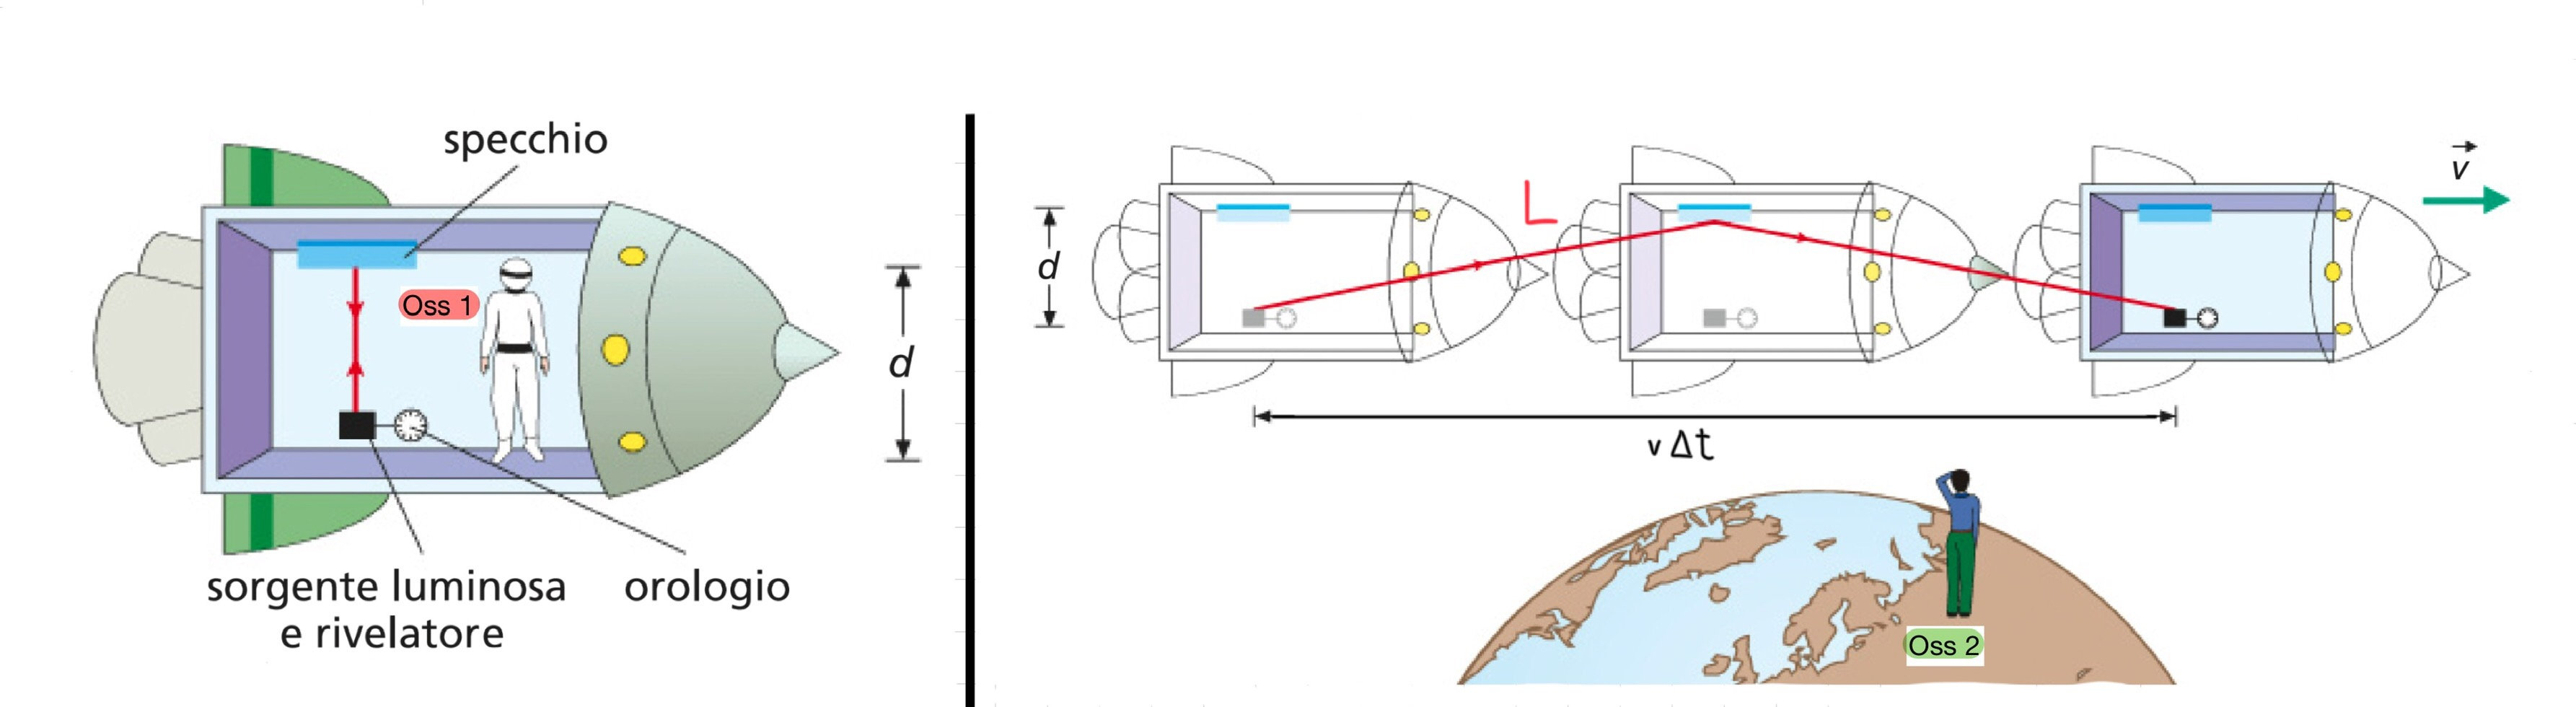
\includegraphics[width=10cm]{img/IMG_0355_2}
\end{center}

Per l'\textbf{osservatore 1} il tempo che intercorre tra quando il raggio parte dalla sorgente a quando ritorna è un tempo proprio, in quanto i due eventi avvengono per lui nello stesso posto. Pertanto
\[\Delta\tau = \frac{2d}{c}\]

Per l'\textbf{osservatore 2} i due eventi (partenza del raggio e ritorno) avvengono in due luoghi diversi, e la luce avrà percorso uno spazio $2L$, e pertanto il tempo da lui misurato sarà $\Delta t$ \textbf{non proprio}.
\begin{multline*}
L=\sqrt{\Bigg(\frac{1}{2}v\,\Delta t\Bigg)^2+d^2}=\sqrt{\Bigg(\frac{1}{2}v\,\Delta t\Bigg)^2+\Bigg(\frac{1}{2}c\,\Delta\tau\Bigg)^2}\\
L^2=\Bigg(\frac{1}{2}v\,\Delta t\Bigg)^2+\Bigg(\frac{1}{2}c\,\Delta\tau\Bigg)^2\\
L^2=\frac{\,\Delta t^2c^2}{4}
\end{multline*}

\begin{multline*}
\frac{\Delta t^2c^2}{4}=\frac{v^2\,\Delta t^2}{4}+\frac{c^2\,\Delta\tau^2}{4}\\
\Delta t^2(c^2-v^2)=c^2\,\Delta\tau^2\\
\Delta t^2=\frac{c^2\,\Delta\tau^2}{(c^2-v^2)}
\end{multline*}

\[\Delta t^2=\frac{\Delta \tau^2}{1-v^2/c^2}\]

\equazione{\Delta t=\frac{\Delta \tau}{\sqrt{1-\frac{v^2}{c^2}}}}

\noindent Siano
\[\gamma=\frac{1}{\sqrt{1-\frac{v^2}{c^2}}}\]
denominato \textbf{fattore di Lorentz}, e
\[\beta=\frac{v}{c}\quad\implies \quad\gamma=\frac{1}{\sqrt{1-\beta^2}}\]
allora
\[\Delta t =\gamma\,\Delta\tau\]
che sintetizza tutte le osservazioni precedenti: la misura del tempo è legata allo stato di quiete o di moto degli osservatori, e gli intervalli di tempo tra due eventi dipendono da quanto questi siano distanti; intervalli di tempo e di spazio sono concatenati.

Siccome vale sempre $\beta<1$, allora $\gamma>1$, e di conseguenza
\[\Delta t>\Delta \tau\]

Per valori piccoli di $v$, $\gamma\approx1$, e pertanto nella vita di tutti i giorni non ci accorgiamo degli effetti relativistici.

\subsubsection{Paradosso dei gemelli}

Immaginiamo che due gemelli siano separati nel giorno del ventesimo compleanno, e che uno venga lanciato nello spazio, ad orbitare attorno alla Terra a velocità poco inferiore a quella della luce ($0,98c$), mentre l’altro viene lasciato sulla Terra.

Ammettiamo che il tempo proprio (misurato dal fratello nello spazio) $\tau$ sia di 10 anni. Secondo la dilatazione del tempo, il tempo $\Delta t$ percepito dal gemello a Terra sarà maggiore, per la precisione:

\[\Delta t=\frac{\Delta\tau}{\sqrt{1-0,98^2}}=50\,\text{anni}\]

Secondo i calcoli, se si incontrassero sulla terra dopo 10 anni, tempo proprio, uno avrebbe 30 anni, mentre l’altro 70.
Questo viene chiamato paradosso, ovvero qualcosa che contrasti il senso comune.

Il paradosso consiste anche nel fatto che come uno viaggia rispetto all’altro con velocità di $0,98c$, anche l’altro fa lo stesso. Questo problema è risolto prendendo in considerazione il fatto che il gemello subisce una doppia accelerazione, una per decollare ed una per atterrare, ed essi non sono quindi in moto relativo costantemente alla stessa velocità.

\subsection{Contrazione delle lunghezze}

Anche la distanza fra due punti, come l'intervallo di tempo fra due istanti, è una grandezza relativa, la cui misura dipende dal moto dell'osservatore.

Si immagini un'astronave in viaggio dalla terra a Plutone, e due osservatori (\textbf{primo osservatore}, sulla terra, e \textbf{secondo osservatore} sull'astronave), considerando i due pianeti fermi dagli osservatori terrestri.

\begin{center}
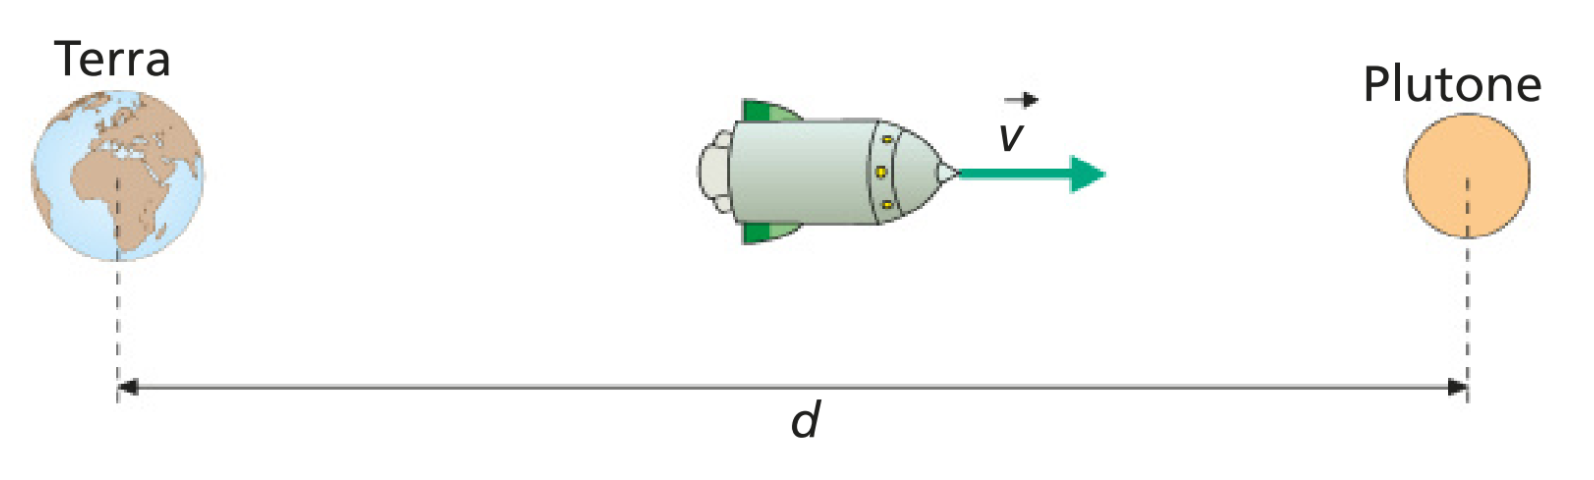
\includegraphics[width=12cm]{img/lunghezza1}
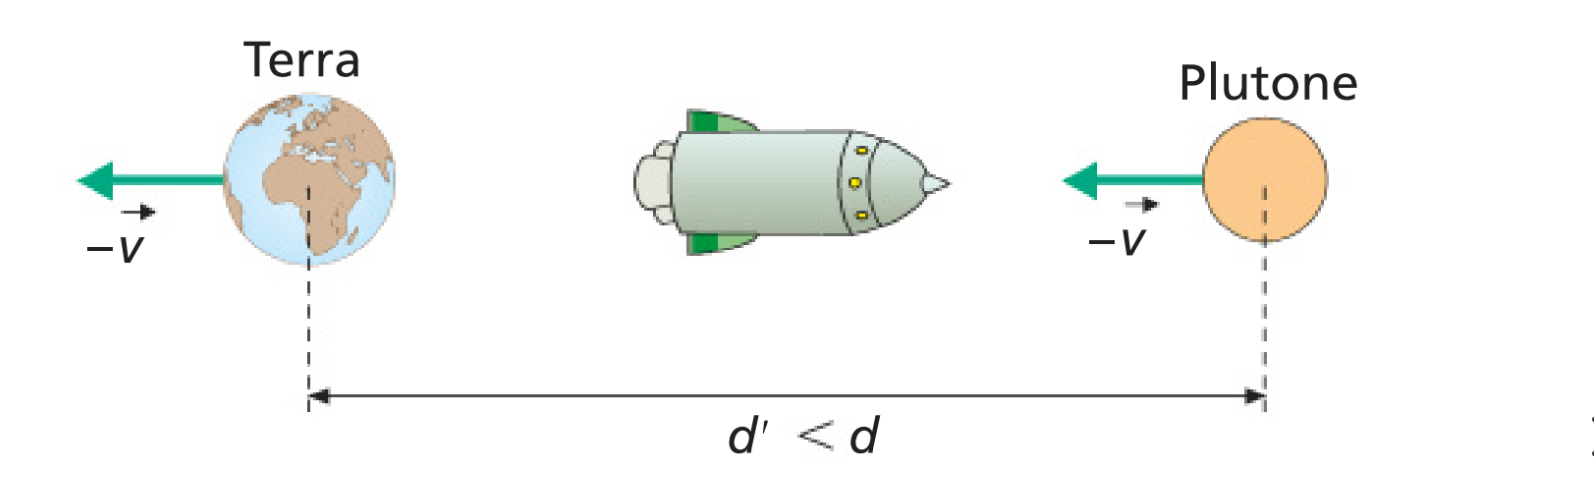
\includegraphics[width=12cm]{img/lunghezza2}
\end{center}

\paragraph{Primo osservatore} La terra e plutone sono separati da una distanza $d$ (lunghezza propria $\mathfrak{L}$, in quanto misurata in un sistema di riferimento fermo rispetto alla stessa), e per percorrerla l'astronave impiegherà un tempo tale che 
\[
d = v \,\Delta t
\]

\paragraph{Secondo osservatore} I due pianeti transitano con velocità $-\vec{v}$, ad un intervallo di tempo $\Delta t'$ l'uno dall'altro (tempo proprio $\Delta \tau$)
\[
\Delta\tau=\Delta t'=\sqrt{1-\frac{v^2}{c^2}}\,\cdot\,\Delta t
\]
Ne deriva che se $d'=v\,\Delta t'$ è la distanza Terra-Plutone rispetto al secondo osservatore, 
\[
d'=v \,\sqrt{1-\frac{v^2}{c^2}} \,\Delta t
\]
e $d = v\,\Delta t$
\[
d' = \sqrt{1-\frac{v^2}{c^2}} \, d
\]

Considerando $d'$ come una qualsiasi lunghezza $L$, e ricordando il fattore di Lorentz, posso scrivere:
\equazione{L=\frac{\mathfrak{L}}{\gamma}}

\subsubsection{La lunghezza propria}

La lunghezza di un segmento, misurata rispetto al sistema di riferimento inerziale in cui questo è fermo, prende il nome di \textbf{lunghezza propria}. La contrazione delle lunghezze si verifica solo nella direzione del moto.

\subsection{Trasformazioni di  Lorentz}

Riprendiamo le trasformazioni di Galileo.
\begin{center}
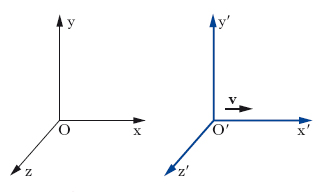
\includegraphics[width=7cm]{img/galileo}
\end{center}
Se il sistema di riferimento $S'$ si muove di velocità $\vec{v}$ parallela all'asse delle $x$ rispetto ad $S$, la distanza $\overline{OO'}=vt$, e le trasformazioni galileiane sono:
\[\begin{cases}
x'=x-vt\\
y'=y\\
z'=z\\
t'=t
\end{cases}\qquad\qquad\begin{cases}
u'_x=u_x-v\\
a'=a
\end{cases}\]

Per queste trasformazioni è necessario un unico orologio, ed invarianti sono il \textbf{tempo} e l'\textbf{accelerazione}.

Per le \textbf{trasformazioni di Lorentz}, invece, nelle stesse condizioni precedenti, valgono le seguenti equazioni
\[\begin{cases}
x'=\gamma\,(x-vt)\\
y'=y\\
z'=z\\
t'=\gamma\,(t-\frac{xv}{c^2})
\end{cases}\qquad\qquad\begin{cases}
x=\gamma\,(x'+vt')\\
y=y'\\
z=z'\\
t=\gamma\,(t'+\frac{x'v}{c^2})
\end{cases}\]
Sono necessari due orologi, uno per ciascun sistema di riferimento.

La più significativa differenza fra le trasformazioni di Galileo e quelle di Lorentz riguarda la coordinata temporale. Mentre nelle prime è $t'=t$, nelle seconde l'istante $t'$ in cui un evento è visto da un osservatore fermo rispetto al sistema $S'$ dipende sia dalla coordinata temporale $t$ sia dalla coordinata spaziale $x$ assegnate all'evento da un osservatore fermo rispetto al sistema $S$. Pertanto, nelle trasformazioni di Lorentz il tempo non è più una grandezza assoluta, ma una grandezza correlata con lo spazio e relativa al sistema di riferimento.

\subsection{Velocità}

Affinché la velocità della luce sia uguale a $c$ in tutti i sistemi di riferimento inerziali e il principio di relatività sia valido per l'elettromagnetismo, oltre che per la meccanica, è necessario formulare non solo nuove trasformazioni per le coordinate spazio-temporali, ma anche una diversa legge di composizione della velocità.

\begin{center}
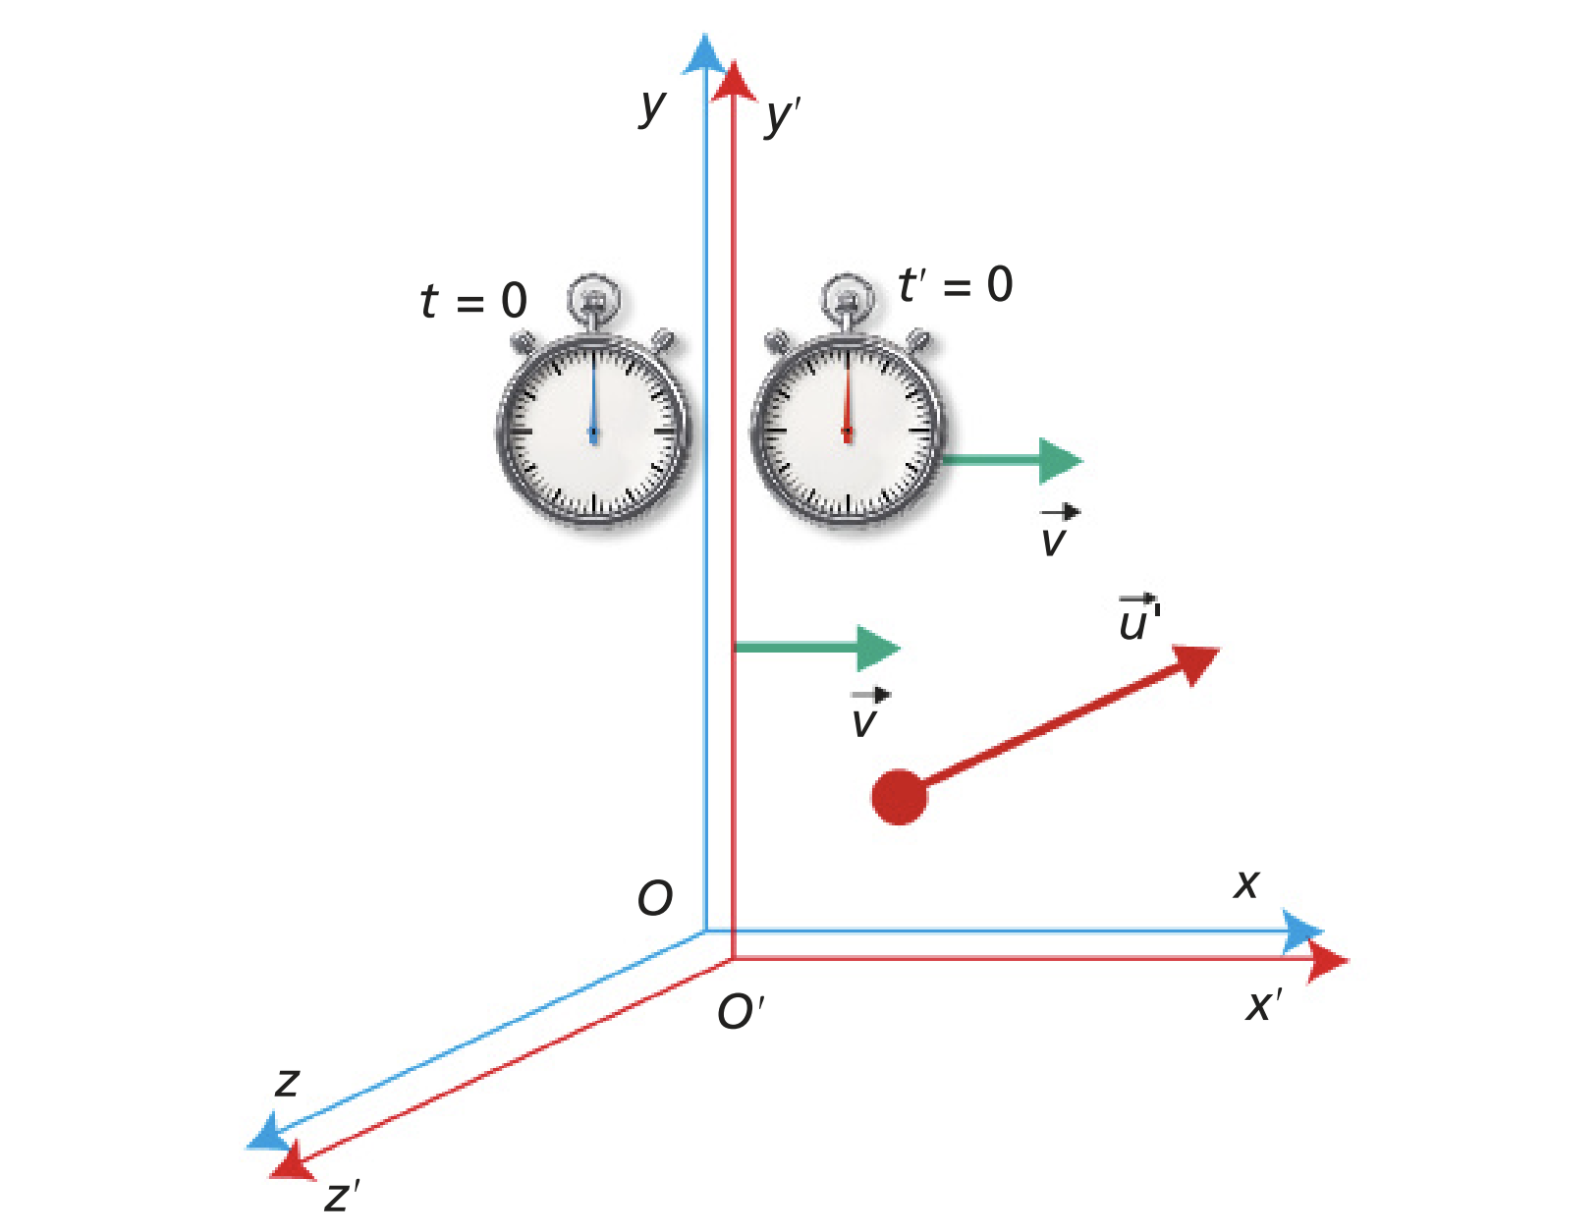
\includegraphics[width=8cm]{img/lorentzvel}
\end{center}

Rispetto a due sistemi di riferimento inerziali $S$ ed $S'$, a uno stesso evento si assegnano rispettivamente, le coordinate spazio-temporali $x$, $y$, $z$, $t$ e $x'$, $y'$, $z'$, $t'$.
Assumiamo che $S'$ sia in moto rispetto a $S$ con velocità $\vec{v}$ lungo la comune direzione degli assi $x$ e $x'$.

Sia $u$ la velocità del corpo rispetto ad $S$, ed $u'$ la velocità dello stesso corpo rispetto ad $S'$

Sia $\vec{u}$ una velocità nel sistema di riferimento $S$, corrispondente ad $\vec{u}'$ nel sistema di riferimento $S'$, composta nelle tre dimensioni ($u_x$, $u_y$, $u_z$ e $u_x'$, $u_y'$, $u_z'$). Per le trasformazioni di Lorenz, dati $u_x=x/t$ e $u_x'=x'/t'$:

\begin{gather*}
x=\gamma\,(x'+v_tt')=\gamma\,(x'/t'+v_t)\,t'=\gamma\,(u_x'+v)\,t'\\
t=\gamma\,\Big(t'+\frac{x'v}{c^2}\Big)=\gamma\,\Big(1+\frac{x'v}{t'\cdot c^2}\Big)\,t'=\gamma\,\Big(1+\frac{u_x'v}{c^2}\Big)\,t'
\end{gather*}
\[u_x=\frac{\gamma\,(u_x'+v)\,t'}{\gamma\,(1+\frac{u_x'v}{c^2})\,t'}=\frac{u_x'+v_t}{1+(u_x'v_t)/c^2}\]

Allo stesso modo si dimostrano anche le due espressioni successive:
\begin{gather*}
u_y=\frac{u_y'\cdot\sqrt{1-v_t^2/c^2}}{1+(u_x'v_t)/c^2}\\
u_z=\frac{u_z'\cdot\sqrt{1-v_t^2/c^2}}{1+(u_x'v_t)/c^2}
\end{gather*}

Applicando lo stesso principio, sempre partendo dalle trasformazioni di Lorentz, si giunge alle formule inverse:
\[u_x'=\frac{u_x-v_t}{1-(u_x'v_t)/c^2}\qquad u_y'=\frac{u_y\cdot\sqrt{1-v_t^2/c^2}}{1-(u_x'v_t)/c^2}\qquad u_z'=\frac{u_z\cdot\sqrt{1-v_t^2/c^2}}{1-(u_x'v_t)/c^2}\]

\subsection{Spazio tempo}

Se nelle trasformazioni di Galileo l'invariante è la lunghezza di un segmento, per quelle di Lorentz non è più così. È possibile formulare alcune ipotesi riguardo a quale possa essere l'invariante:
\begin{itemize}
\item $x^2+y^2+z^2+t^2=d^2$: non può essere invariante in quanto non ha una dimensione omogenea;
\item $x^2+y^2+z^2+c^2t^2=d^2$: a differenza dell'invariante precedente questa è omogenea, ma non può essere invariante per la dimostrazione seguente:
\end{itemize}

\paragraph{Dim.} Consideriamo l'invariante $\Delta s^2=\Delta x^2+\Delta y^2+\Delta z^2+c^2\,\Delta t^2$, con $\Delta y = \Delta z = 0$.
\[
\Delta s^2 = \Delta x^2 + c^2\,\Delta t^2
\]
Dato un sistema in moto $S'$ in cui viene azionato un raggio laser due volte, con un intervallo di tempo $\Delta t'=\Delta \tau$, consideriamo questa quantità per un osservatore fermo e per uno concorde a $S'$.
Se fosse realmente invariante, $\Delta s^2 = \Delta s'^2$. Verifichiamolo.

Per l'osservatore fermo
\begin{multline*}
\Delta s^2 = \Delta x^2 + c^2\,\Delta t^2 = \\
= c^2\,\Delta t^2 \Big(\frac{\Delta x^2}{c^2\,\Delta t^2}+ 1\Big) = \\
= c^2\,\Delta t^2 \Big(\frac{v^2}{c^2}+1\Big)
\end{multline*}

Per l'osservatore in moto:
\begin{multline*}
\Delta s'^2 = \Delta x'^2 + c^2\,\Delta t'^2 = \\
= 0 + c^2\,\Delta \tau^2 = \\
= c^2\,\Delta \tau^2
\end{multline*}

Notiamo che dovrebbe valere la condizione:
\[
c^2\,\Delta \tau^2 = c^2\,\Delta t^2 \Big(\frac{v^2}{c^2}+1\Big)\quad\implies\quad\Delta\tau^2 = \,\Delta t^2 \Big(\frac{v^2}{c^2}+1\Big)
\]
che però non è corretta, in quanto la legge della dilatazione dei tempi è:
\[\Delta\tau^2 = \,\Delta t^2 \Big(\frac{v^2}{c^2}-1\Big)\]

Possiamo pertanto intuire che l'invariate corretta sia:
\equazione{\Delta s^2 =\Delta  x^2+\Delta y^2+\Delta z^2-(c\,\Delta  t)^2}

\paragraph{Dim.} Assumiamo per semplicità che uno dei due eventi considerati sia nell'origine dello spazio tempo, comune ai due sistemi. Ne consegue che:
\begin{gather*}
\Delta s^2 =x^2+ y^2+z^2-(ct)^2\\
\Delta s'^2 =x'^2+ y'^2+z'^2-(ct')^2
\end{gather*}

Per le trasformazioni di Lorentz si avrà che:
\[
x^2=\gamma^2(x'+vt')^2=\frac{x'^2+2vx't'+v^2t'^2}{1-v^2/c^2};\quad y^2 = y'^2;\quad z^2=z'^2
\]
\[
(ct)^2=\Big[\gamma\, c\,\Big(t'+\frac{vx'}{c^2}\Big)\Big]^2=\frac{c^2t'^2+2vx't'+\frac{v^2x'^2}{c^2}}{1-v^2/c^2}
\]
da cui
\begin{multline*}
x^2+ y^2+z^2-(ct)^2 = \\
= \frac{x'^2+2vx't'+v^2t'^2}{1-v^2/c^2} + y'^2 + z'^2 - \frac{c^2t'^2+2vx't'+\frac{v^2x'^2}{c^2}}{1-v^2/c^2} = \\
= \frac{c^2\Big(x'^2+\cancel{2vx't'}+v^2t'^2-c^2t'^2-\cancel{2vx't'}-\frac{v^2x'^2}{c^2}\Big)}{c^2-v^2} + y'^2 + z'^2 = \\
= \frac{c^2x'^2+c^2v^2t'^2-c^4t'^2-v^2x'^2\Big)}{c^2-v^2} + y'^2 + z'^2 = \\
= \frac{(c^2-v^2)(x'^2-c^2t'^2)}{c^2-v^2}+ y'^2 + z'^2 = \\
= \frac{\cancel{(c^2-v^2)}(x'^2-c^2t'^2)}{\cancel{c^2-v^2}}+ y'^2 + z'^2 = \\
= x'^2+ y'^2+z'^2-(ct')^2 \qed
\end{multline*}
\end{document}